\section{Method}
\subsection{Deep Deterministic Policy Gradient}
Deep Deterministic Policy Gradient is an off-policy actor-critic algorithm that uses a replay buffer and two target networks \cite{DDPG}. In each training cycle, the agent rollouts some  transition datas from the environment $E$ and stores them into the replay buffer $D$. Then calculate the Bellman Error by equation (\ref{eq:bellman}) with the target network $Q'$ and $\mu'$ and optimize the parameters $\theta^{Q}$ of the critic $Q$ in several training steps. And optimize the parameters $\theta^{\mu}$ of the actor $\mu$ by the policy gredient estimated by the critic. The target network is soft updated at the end of each training step. The details of the algorithm are described in Alg \ref{alg:DDPG}.
\begin{equation}
   \label{eq:bellman} 
   \begin{aligned}
   L^Q=\mathbb{E}_{s_t\sim\rho^{\tilde\mu},a_t\sim\tilde\mu,r_t\sim E}[(Q(s_t,a_t)-y_t)^2]\\
   \text{where\quad}  y_t = Q'(s_{t+1},\mu'(s_{t+1}))+r_t
   \end{aligned}
\end{equation}

Since DDPG is an off policy algorithm, the rollout actor and the learning actor do not need to be the same, the exploration strategy $f(\cdot) : \mathbb{M} \rightarrow \mathbb{M}$, which $\mathbb{M}$ is the space of policy, commonly transforms the learning actor $\mu$ into a rollout actor $\tilde\mu$ to achieve exploration.

\begin{algorithm}[htbp]
   \caption{Deep Deterministic Policy Gradient}
   \label{alg:DDPG}
\begin{algorithmic}
   \STATE {\bfseries Input:} environment $E$, critic $Q(s,a|\theta^Q)$, actor $\mu(s|\theta^\mu)$, exploration strategy $\tilde\mu \leftarrow f(\mu)$
   \STATE Initialize replay buffer $D = \emptyset$.
   \STATE Initialize target network $Q'= Q$, $\mu'= \mu$.
   \FOR{1 {\bfseries to} cycle\_number}
   \STATE Apply exploration strategy $\tilde\mu \leftarrow f(\mu)$
   \STATE Rollout data $d_t$ from $E$ by $\tilde\mu$ and $D \leftarrow D\cup {d_t}$

   \FOR{1 {\bfseries to} train\_steps}
   \STATE Sample data batch $\{d_t=(s_t,a_t,r_t)\}$ from $D$
   \STATE $L^Q=\sum(Q'(s_{t+1},\mu'(s_{t+1}))+r_t-Q(s_t,a_t))^2$
   \STATE $L^\mu=-\sum Q(\mu(s_t))$
   \STATE $\theta^Q \leftarrow \theta^Q - \alpha^Q\cdot\nabla_{\theta^Q} L^Q$
   \STATE $\theta^\mu \leftarrow \theta^\mu -\alpha^\mu\cdot\nabla_{\theta^\mu} L^\mu$
   \STATE Soft update target network $Q'$ and $\mu'$
   \ENDFOR
   \ENDFOR
\end{algorithmic}
\end{algorithm}

\subsection{Stochastic Gradient Langevin Dynamic}
Stochastic Gradient Langevin Dynamic algorithm  is an algorithm that can perform MCMC sampling on a large dataset in stochastic gradient way \cite{SGLD}. For a paramter vector $\theta$ with a prior distribution $p(\theta)$ ,to draw a sample chain $\{\theta_1,\theta_2,\cdots\}$ follow $p(\theta|D)$ where $D=\{d_i\}^N_{i=1}$, the parameters should be updated as follow:
\begin{equation}
   \label{eq:sgld} 
   \begin{aligned}
\Delta\theta =\frac{\epsilon}{2}\frac{N}{n}\sum_{i=1}^{n}\nabla_\theta\log p(d_i|\theta)+\frac{\epsilon}{2}\nabla_\theta\log p(\theta)\\
+\mathcal{N}(0,\epsilon)
\end{aligned}
\end{equation}
Where $\epsilon$ is the learning rate, $n$ is the size of one mini-batch. 

The basic SGLD algorithm updates all parameters with the same step size, which leads to slow mixing rate. In practical, we use preconditioned SGLD (pSGLD) instead, in which the step size is scaled by preconditioner $G_t$ as follow:
\begin{equation}
   \label{eq:psgld} 
   \begin{aligned}
      \Delta\theta =\frac{\epsilon}{2}\frac{N}{n}G_t\sum_{i=1}^{n}\nabla_\theta\log p(d_i|\theta)+\frac{\epsilon}{2}G_t\nabla_\theta\log p(\theta)\\
      +\mathcal{N}(0,\epsilon G_t)
   \end{aligned}
\end{equation}
Where $G_t$ is updated as the mean square term in RMSprop \cite{rmsprop}.

%$\nabla_\theta p(d_i|\theta)$ is the data like-hood term, which corresponding to gradient of loss. $\nabla_\theta p(\theta)$ is prior probability term, it is equivalent to L2 regularization if $p(\theta)\sim\mathcal{N}(0,\sigma^2)$. And $\mathcal{N}(0,\epsilon)$ term make SGLD can sample parameters with $\theta \sim p(\theta|D)$
To visualize the ability of pSGLD to characterization the uncertainty of posterior distribution when fitting data set, we trained a neural network with architecture of "20-ReLU-20-ReLU-1" by pSGLD on three toy datasets, left: $y=0$, mid: $y=-x^2$, right: $y=x^3-x$, and the results are shown in the figure \ref{fig:three}. The dark curve is the average of the curve clusters, and the light areas represent the standard deviation of the curve clusters. The results show that the curve samples of pSGLD are concentrated near the data points, while diverge in both positive and negative directions in areas far from the data, even on the all zero data set.
\begin{figure*}[htbp]
   \begin{center}
      \centerline{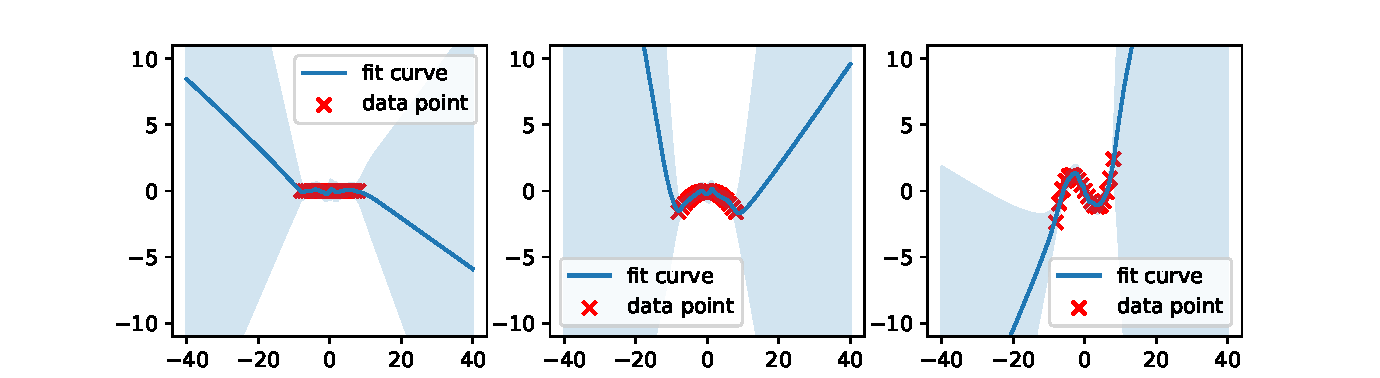
\includegraphics[width=480pt]{figs/three-curve}}
   \caption{The results of curve fitting by using pSGLD on three toy data sets.}
   \label{fig:three}
   \end{center}
\end{figure*}

\subsection{SGLD in DDPG}
In baseline DDPG algorithm, the parameters of critic network $\theta^Q$ is updated by an Adam optimizer to minimize the Bellman error $L^Q$. To replace the Adam optimizer by pSGLD sampler with minimal changes, we suppose that the likelihood term is $p(d_i|\theta^Q)\sim\exp(-L^Q)$ to match the Bellman error, and prior term is $p(\theta^Q)\sim \mathcal{N}(0,\sigma^2)$ to match the L2 regularization on critic network. Then the critic will updated as follow :
\begin{equation}
   \label{eq:rlpsgld} 
   \begin{aligned}
      \Delta\theta^Q =-\frac{\epsilon}{2}\frac{N}{n}G_t\sum_{i=1}^{n}\nabla_\theta L^Q -\frac{\epsilon}{2}G_t \frac{\theta^Q}{\sigma^2}\\
      +\mathcal{N}(0,\epsilon G_t)
   \end{aligned}
\end{equation}
It is worth noting that, unlike supervised learning, the size of data sets $N$ in reinforcement learning is increasing as the training process increases. If the learning rate $\epsilon$ remains constant, the gradient of the likelihood term will continue to grow, resulting in an unstable training process. In order to keep the training process stable, we implement learning rate decay as opposed to data set size growth: $\epsilon_t=\frac{n}{N}\epsilon_0$. Now the equation (\ref{eq:rlpsgld}) turns into:
\begin{equation}
   \label{eq:rlpsgld1} 
   \begin{aligned}
      \Delta\theta^Q =-\frac{\epsilon_0}{2}G_t\sum_{i=1}^{n}\nabla_\theta L^Q -\frac{\epsilon_0}{2}\frac{n}{N}G_t \frac{\theta^Q}{\sigma^2}\\
      +\mathcal{N}(0,\epsilon_0\frac{n}{N} G_t)
   \end{aligned}
\end{equation}
The observed data is increasing as the learning process progresses, which leads to the effect of the prior term and the noise term becomes weaker than the likelihood term. This is consistent with our common sense: the more data is observed, the more the model's distribution is concentrated toward the maximum likelihood estimate.



\subsection{Further follow posterior distribution}
In original DDPG algorithm, the target networks are the $\tau$-moving average of parameters of actor and critic. After each gradient descent step on actor and critic ,the target networks are "soft updated" by equation (\ref{eq:soft}).
\begin{equation}
\label{eq:soft} 
\begin{aligned}
\theta^{Q'} = (1-\tau)\theta^{Q'}+\tau\theta^Q\\
\theta^{\mu'} = (1-\tau)\theta^{\mu'}+\tau\theta^\mu
\end{aligned}
\end{equation}

The optimized object for the critic in one cycle is minimizing Bellman error in equation (\ref{eq:bellman}), which is associated with both data in replay buffer and the target network. Constantly updating the target during the training step will make the process of sampling from the posterior distribution inconsistently. In order to sample critic from posterior distribution more strictly, we remain the target unchanged in one cycle and do "hard update",directly copy parameters of actor and critic to target networks. Under this setting, the expectation policy gradient will be intergrated over both $s_t\sim\rho$ and $\theta^Q\sim p(\theta^Q|D)$ as equation (\ref{eq:pg}). 
\begin{equation}
   \label{eq:pg} 
   \begin{aligned}
   \nabla_{\theta^\mu}\mathbb{E}[L^\mu|D] = \mathbb{E}_{s_t\sim\rho,\theta^Q\sim p(\theta^Q|D)}[\nabla_{\theta^\mu}L^\mu]\\
   \end{aligned}
\end{equation}
It is proven to be the correct form to estimate policy gradient with critics sampled from posterior distribution in \cite{henderson2017bayes}.
   